% presentation
\documentclass{beamer}

% \usetheme{Boadilla}
\usetheme{Warsaw}

% rus lang
\usepackage[main=russian,english]{babel}

% insert images
\usepackage{wrapfig}
\usepackage{graphicx}
\graphicspath{{./img/}, {../../plots/}}

% declare operator
\DeclareMathOperator*{\argmin}{argmin} % thin space, limits underneath in displays
\newcommand{\at}[2][]{#1|_{#2}}
\newcommand{\eps}{\varepsilon}

% math
\usefonttheme[onlymath]{serif}
\newtheorem{rustheorem}{Теорема}
\usepackage{amsmath}
\DeclareMathOperator{\sign}{sign}
\DeclareMathOperator{\K}{K}
\DeclareMathOperator{\R}{\mathbb{R}}
\DeclareMathOperator{\X}{\mathbb{X}}
\DeclareMathOperator{\Y}{\mathbb{Y}}
\DeclareMathOperator{\E}{\mathbb{E}}
\DeclareMathOperator{\V}{\mathbb{V}}


\title[Ансамбли]{Лекция 7. Композиции алгоритмов}
\subtitle{Основы интеллектуального анализа данных}
\author{Полузёров Т. Д.}
\institute{БГУ ФПМИ}
\date{}

\begin{document}
	
	\begin{frame}
		\titlepage
	\end{frame}
	
	
	\begin{center}
		\frametitle{Структура лекции}
		\tableofcontents
	\end{center}
	
	\section{Беггинг}

	\begin{frame}
		\frametitle{Функионал риска}
		Рассмотрим задачу регрессии с квадратичной функцией потерь. Качество алгоритма $a$:
		\[
		Q(a) = \E_x \E_{X, \eps} [y(x, \eps) - a(x, X)]^{2}
		\]

		\begin{itemize}
			\item $X$ --- обучающая выборка
			\item $y = f(x) + \eps$ --- целевая зависимость, наблюдаемая с точностью до шума $\eps$
			\item $a(x, X)$ --- ответ алгоритма в точке $x$, обученного по выборке $X$
			\item $\E_x$ --- среднее по всем тестовым точкам, 
			\item $\E_{X, \eps}$ --- среднее по всем обучающим выборкам и случайному шуму
		\end{itemize}
	\end{frame}

	\begin{frame}
		\frametitle{Смещение и разброс}
		
		Ошибку можно предстваить в виде трех слагаемых:
		\[
		Q(a) = \E_x bias_X^2 (a) + 
		\E_x variance_X (a)
		+ \sigma^2
		\]
		где
		\begin{itemize}
			\item $bias_X(a) = f(x) - \E_x [a(x, X)]$ --- смещение
			\item $variance(a) = \E_X [ a(x, X) - \E_x[a(x, X)] ]^2$ --- разброс
			\item $\sigma^2 = \E_x \E_{\eps} [y(x, \eps) - f(x)]^2$ --- неустранимый шум
		\end{itemize}
	\end{frame}

	\begin{frame}
		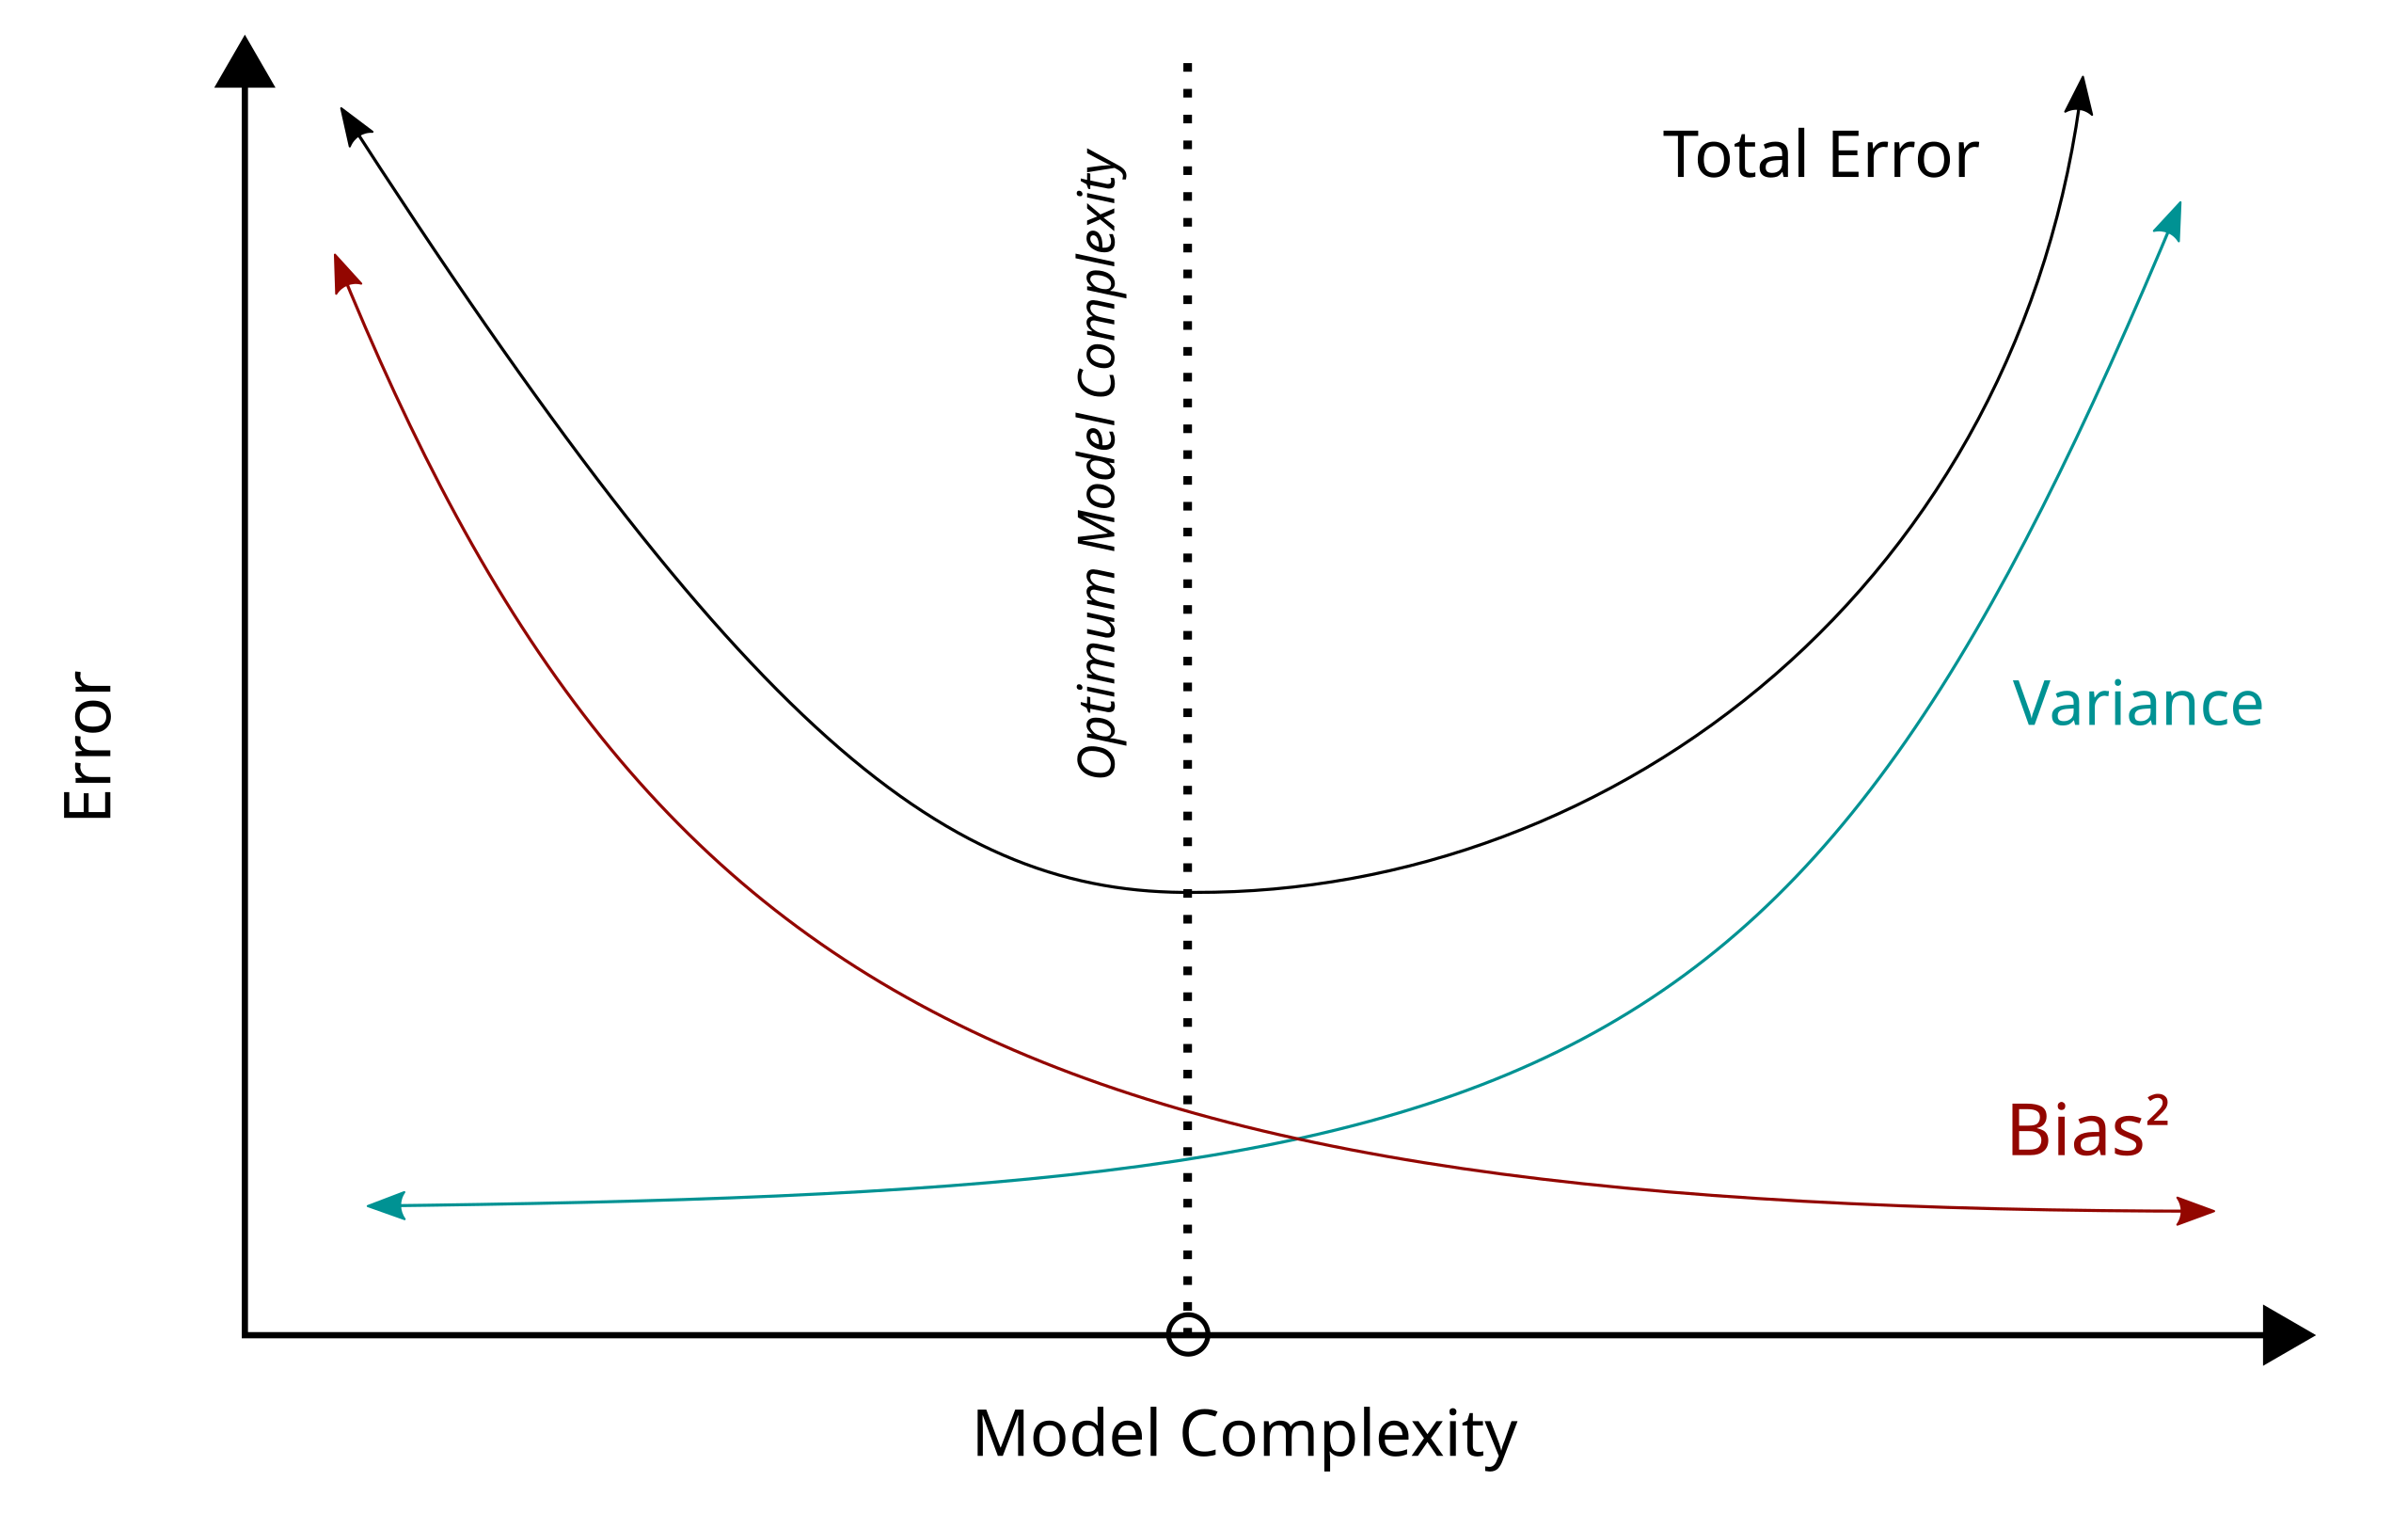
\includegraphics[width=1\textwidth]{img/bias_variance_tradeoff.png}	
	\end{frame}

	\begin{frame}
		\frametitle{Бутстреп}

		Пусть имеется выборка $X$ объема $\ell$.

		\vspace{15pt}

		С помощью \textbf{выбора с возвращением} сформируем новую <<выборку>> $X^1$ тоже объема $\ell$. 

		Проделаем эту операцию $k$ раз и получим $\{X^1, \dots, X^k\}$ \textbf{псевдовыборок}.

		\vspace{15pt}

		Такой метод получения псевдовыборок называется \textbf{бутстрепом} (bootstrap).

		\vspace{15pt}

		Применяется в статистике для проверки гипотез, построения доверительных интервалов \dots
	\end{frame}

	\begin{frame}
		\frametitle{Бэггинг}
		
		Сгенерируем $k$ псевдовыборок $\{X^1, \dots, X^k\}$ и обучим на каждой из них базовую модель $b$.
		
		Получим $k$ обученных алгоритмов $b_i(x) = b_i(x, X^i), i=1, \dots, k$.

		Итговый алгоритм есть голосование базовых

		\[
		a(x) = \frac{1}{k} \left( b_1(x) + \dots + b_k(x) \right)
		\]
		Такой ансамбль алгоритмов --- \textbf{бэггинг} (bagging, bootstrap aggregation)	
	\end{frame}
	
	\begin{frame}
		\frametitle{Смещение бэггинга}

		\begin{align*}
			bias_X(a) = 
			f(x) - \E_X[a(x, X)] = \\
			= f(x) - \E_X \left[\sum_{i=1}^{k} \frac{1}{k} b(x, X^i) \right] = \\
			= f(x) - \E_X b(x, X) = \\
			= bias_X(b)
		\end{align*}

		Смещение ансамбля определяется смещением базового алгоритма.
	\end{frame}

	\begin{frame}
		\frametitle{Разброс бэггинга}

		\begin{align*}
			variance_X(a) & = \E_X [ a(x, X) - \E_x[a(x, X)] ]^2 = \\
			& = \E_X \left[ \frac{1}{k} \sum_{i=1}^{k} b_i - \E_X \left[ \frac{1}{k} \sum_{i=1}^{k} b_i \right] \right]^2 = \\
			& = \frac{1}{k^2} \E_X \left[ \sum_{i=1}^{k} \left( b_i - \E_X b_i \right) \right]^2 = \\
			& = \frac{1}{k^2} \sum_{i=1}^{k} variance_X(b_i) + 
			\frac{1}{k^2} \sum_{i \ne j} cov(b_i, b_j)
		\end{align*}
	\end{frame}

	\begin{frame}
		\frametitle{}

		В случае если базовые алгоритмы некоррелированны, то

		\begin{align*}
			variace_X(a) = \frac{1}{k^2} \sum_{i=1}^{k} variance_X(b_i) = \\ 
			= \frac{1}{k^2} \sum_{i=1}^{k} variance_X(b) = \\
			= \frac{1}{k} variance_X(b)
		\end{align*}

		Используя некоррелированную композицию алгоритмов, можно добиться уменьшения разброса 
		в $k$ раз!
	\end{frame}

	\begin{frame}
		\frametitle{Случайный лес}

		На практике строгое выполнение требования некоррелированности --- необяязательно,
		достаточно, чтобы базовые алгоритмы были непохожи друг на друга.

		\vspace{15pt}

		Посмтроим бэггинг над решающими деревьями
		\begin{enumerate}
			\item Построение $i$-го дерева
			\begin{itemize}
				\item сэмплируется псевдовыборка $X^i$
				\item в процессе построения дерева, в каждой вершине выбирается $n^{'} < n$ признаков и по ним ищется сплит
				(метод случайных подпространств)
			\end{itemize}
			\item итоговый ответ ансамбля: среднее для задач регрессии,
			наиболее популярный класс для классификации
		\end{enumerate}
	\end{frame}

	\begin{frame}
		\frametitle{Случайный лес}

		Бэггинг над решающими дереьями --- случайный лес (random forest).

		Непохожесть алгоритмов получается за счет обучения на разных псевдовыборках
		и использовании метода случайных подпространств.

		\vspace{15pt}

		Остаются вопросы
		\begin{itemize}
			\item Какой глубины $h$ строить деревья?
			\item Сколько признаков $n^{'}$ использовать для обучения?
			\item Сколько деревьев $k$ использовать в композиции?
		\end{itemize}
	\end{frame}

	\begin{frame}
		\frametitle{Глубина деревьев}

		Ошибка состоит из смещения и разброса.
		Разброс снижается за счет композиции, а смещение определяется смещением базового дерева.

		Поэтому необходимо использовать \textbf{деревья с низким смещением}.
		\begin{itemize}
			\item Неглубокие деревья имеют малое число параметров и поэтому строят только верхнеуровневые зависимости.
			При разных обучающих подвыборках алгоритмы не будут значительно отличатся (низкий разброс, высокое смещение).
			\item Глубокие деревья наоборот чересчур сильно подстраиваются под данные, поэтому имеют сильный разброс, но низкое смещение.
		\end{itemize}
		\vspace{15pt}

		Используем \textbf{глубокие деревья}.
	\end{frame}

	\begin{frame}
		\frametitle{Число признаков}

		Большое число признаков обеспечивает слабое различие деревьев, поэтому эффект
		от бэггинга --- слабый.

		С другой стороны, используя малое число признаков, базовые деревья будут слабыми.

		\vspace{15pt}

		Практическая рекомендация:
		\begin{itemize}
			\item Для задач регрессии --- $n^{'} = n / 3$
			\item Для задач классификации --- $n^{'} = \sqrt{n}$
		\end{itemize}
	\end{frame}

	\begin{frame}
		\frametitle{Размер ансамбля}

		С ростом числа деревьев снижается разброс, но число признаков и вариантов подвыборок --- ограничены.
		Поэтому бесконечно уменьшать разброс не получится.

		\vspace{15pt}

		Имеет смысл построить график зависимости ошибки от числа деревьев и остановиться в тот момент, когда
		ошибка перестанет значимо уменьшатся

		\vspace{15pt}

		Так же ограничением может выступать время работы ансамбля. Большее число деревьев --- большее время принятия решения.

		Однако, алгоритмы стоятся независимо друг от друга и это позволяет распаралеливать построение отдельных деревьев.
	\end{frame}

	\section{Бустинг}

	\begin{frame}
		\frametitle{Бустинг}
		Задана функция потерь $L(a) = (y - a(x))^2$

		Будем строить последовательно линейную композицию
		\[
		a(x) = b_1(x) + \dots + b_k(x)
		\]
		исходя из следующих соображений.
		
		Допустим, на шаге $t-1$  имеем композицию $a_{t - 1}$. Она допускает ошибки
		$s_{t-1} = y - a_{t-1}$.

		Если дополнить композицию $a_t(x) = a_{t - 1} + s_{t-1}$ --- такой алгоритм решит задачу точно.

		Попробуем строить следующий базовый алгоритм $b_t(x)$ который <<испрвялет>> ошибки, допущенные 
		предыдущей композицией
	\end{frame}

	\begin{frame}
		\frametitle{}
		 
		Требуем от добавления алгоритма к композиции
		\[
		Q(a_k) < Q(a_{k-1})
		\]

		Более подробно
		\[
		Q(a_k) = \sum_{i=1}^{\ell} \mathcal{L} \left( \sum_{j=1}^{k - 1} b_j(x_i) + b_k(x_i), y_i \right) \rightarrow \min_{b}
		\]

		\begin{center}
			$a_0$ --- начальное приближение
	
			$a_1 = a_0 + b_1$ 
			
			$\cdots$

			$a_t = a_{t-1} + b_t$ 
		\end{center}
		Очень похоже на градиентный спуск
		\[
		b_t = - \nabla \mathcal{L}  (a_{t-1})
		\]

	\end{frame}

	\begin{frame}
		\frametitle{}
		Будем строить $b_t$, приближающий антиградиент $\mathcal{L}$ в точке $a_{t-1}$.

		\[
		b_t(x) = \arg \min_{b} \sum_{i=1}^{\ell} (b(x_i) + \nabla \mathcal{L}  (a_{t-1}))^2
		\]

		В градиентных метод оптимизации строится релаксационная последовательность весов, а в градиентном бустинге ---
		последовательность композиций.

	\end{frame}

	\begin{frame}
		\frametitle{Градиентный шаг}

		Бывает полезным ввести параметр --- \textbf{темп обучения}

		А именно делать градиентный шаг
		\[
		a_t(x) = a_{t-1}(x) + \eta_t b_t(x)
		\]
		величиной $\eta_t$.

		Это позволит делать более точную подстройку.

		\vspace{15pt}

		На $t$-м шаге вычислять $\eta_t$ из решения задачи
		\[
		\eta_t = \arg \min_{\eta > 0} \sum_{i=1}^{\ell} \mathcal{L} (a_{t-1} + \eta b_t(x_i), y_i)
		\]
	\end{frame}


\end{document}

